% Created by tikzDevice version 0.8.1 on 2015-04-03 10:36:45
% !TEX encoding = UTF-8 Unicode
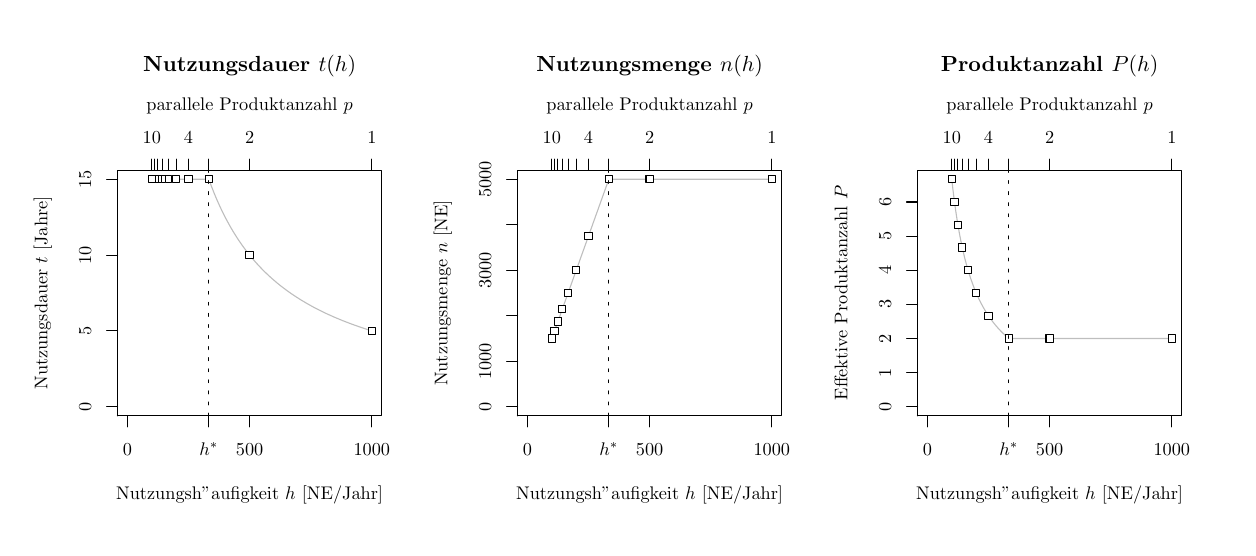
\begin{tikzpicture}[x=1pt,y=1pt]
\definecolor{fillColor}{RGB}{255,255,255}
\path[use as bounding box,fill=fillColor,fill opacity=0.00] (0,0) rectangle (433.62,180.67);
\begin{scope}
\path[clip] ( 32.47, 40.39) rectangle (127.91,129.19);
\definecolor{drawColor}{RGB}{190,190,190}

\path[draw=drawColor,line width= 0.4pt,line join=round,line cap=round] (124.37, 71.09) --
	(120.55, 72.33) --
	(117.04, 73.57) --
	(113.82, 74.81) --
	(110.84, 76.05) --
	(108.08, 77.29) --
	(105.51, 78.53) --
	(103.12, 79.77) --
	(100.90, 81.01) --
	( 98.81, 82.25) --
	( 96.85, 83.49) --
	( 95.02, 84.72) --
	( 93.29, 85.96) --
	( 91.66, 87.20) --
	( 90.11, 88.44) --
	( 88.66, 89.68) --
	( 87.27, 90.92) --
	( 85.96, 92.16) --
	( 84.72, 93.40) --
	( 83.53, 94.64) --
	( 82.40, 95.88) --
	( 81.33, 97.12) --
	( 80.30, 98.36) --
	( 79.32, 99.60) --
	( 78.38,100.84) --
	( 77.48,102.08) --
	( 76.62,103.32) --
	( 75.79,104.56) --
	( 75.00,105.80) --
	( 74.23,107.04) --
	( 73.50,108.28) --
	( 72.80,109.52) --
	( 72.12,110.76) --
	( 71.46,112.00) --
	( 70.83,113.23) --
	( 70.22,114.47) --
	( 69.63,115.71) --
	( 69.06,116.95) --
	( 68.51,118.19) --
	( 67.98,119.43) --
	( 67.46,120.67) --
	( 66.97,121.91) --
	( 66.48,123.15) --
	( 66.02,124.39) --
	( 65.56,125.63) --
	( 65.12,125.91) --
	( 64.69,125.91) --
	( 64.28,125.91) --
	( 63.88,125.91) --
	( 63.48,125.91) --
	( 63.10,125.91) --
	( 62.73,125.91) --
	( 62.37,125.91) --
	( 62.02,125.91) --
	( 61.68,125.91) --
	( 61.35,125.91) --
	( 61.02,125.91) --
	( 60.70,125.91) --
	( 60.40,125.91) --
	( 60.10,125.91) --
	( 59.80,125.91) --
	( 59.52,125.91) --
	( 59.24,125.91) --
	( 58.96,125.91) --
	( 58.70,125.91) --
	( 58.44,125.91) --
	( 58.18,125.91) --
	( 57.93,125.91) --
	( 57.69,125.91) --
	( 57.45,125.91) --
	( 57.22,125.91) --
	( 56.99,125.91) --
	( 56.77,125.91) --
	( 56.55,125.91) --
	( 56.34,125.91) --
	( 56.13,125.91) --
	( 55.92,125.91) --
	( 55.72,125.91) --
	( 55.52,125.91) --
	( 55.33,125.91) --
	( 55.14,125.91) --
	( 54.96,125.91) --
	( 54.77,125.91) --
	( 54.60,125.91) --
	( 54.42,125.91) --
	( 54.25,125.91) --
	( 54.08,125.91) --
	( 53.91,125.91) --
	( 53.75,125.91) --
	( 53.59,125.91) --
	( 53.43,125.91) --
	( 53.28,125.91) --
	( 53.13,125.91) --
	( 52.98,125.91) --
	( 52.83,125.91) --
	( 52.69,125.91) --
	( 52.55,125.91) --
	( 52.41,125.91) --
	( 52.27,125.91) --
	( 52.14,125.91) --
	( 52.01,125.91) --
	( 51.88,125.91) --
	( 51.75,125.91) --
	( 51.62,125.91) --
	( 51.50,125.91) --
	( 51.38,125.91) --
	( 51.26,125.91) --
	( 51.14,125.91) --
	( 51.02,125.91) --
	( 50.91,125.91) --
	( 50.80,125.91) --
	( 50.69,125.91) --
	( 50.58,125.91) --
	( 50.47,125.91) --
	( 50.36,125.91) --
	( 50.26,125.91) --
	( 50.15,125.91) --
	( 50.05,125.91) --
	( 49.95,125.91) --
	( 49.85,125.91) --
	( 49.76,125.91) --
	( 49.66,125.91) --
	( 49.56,125.91) --
	( 49.47,125.91) --
	( 49.38,125.91) --
	( 49.29,125.91) --
	( 49.20,125.91) --
	( 49.11,125.91) --
	( 49.02,125.91) --
	( 48.94,125.91) --
	( 48.85,125.91) --
	( 48.77,125.91) --
	( 48.69,125.91) --
	( 48.60,125.91) --
	( 48.52,125.91) --
	( 48.44,125.91) --
	( 48.36,125.91) --
	( 48.29,125.91) --
	( 48.21,125.91) --
	( 48.13,125.91) --
	( 48.06,125.91) --
	( 47.99,125.91) --
	( 47.91,125.91) --
	( 47.84,125.91) --
	( 47.77,125.91) --
	( 47.70,125.91) --
	( 47.63,125.91) --
	( 47.56,125.91) --
	( 47.49,125.91) --
	( 47.43,125.91) --
	( 47.36,125.91) --
	( 47.29,125.91) --
	( 47.23,125.91) --
	( 47.16,125.91) --
	( 47.10,125.91) --
	( 47.04,125.91) --
	( 46.98,125.91) --
	( 46.92,125.91) --
	( 46.85,125.91) --
	( 46.79,125.91) --
	( 46.74,125.91) --
	( 46.68,125.91) --
	( 46.62,125.91) --
	( 46.56,125.91) --
	( 46.51,125.91) --
	( 46.45,125.91) --
	( 46.39,125.91) --
	( 46.34,125.91) --
	( 46.28,125.91) --
	( 46.23,125.91) --
	( 46.18,125.91) --
	( 46.12,125.91) --
	( 46.07,125.91) --
	( 46.02,125.91) --
	( 45.97,125.91) --
	( 45.92,125.91) --
	( 45.87,125.91) --
	( 45.82,125.91) --
	( 45.77,125.91) --
	( 45.72,125.91) --
	( 45.67,125.91) --
	( 45.63,125.91) --
	( 45.58,125.91) --
	( 45.53,125.91) --
	( 45.49,125.91) --
	( 45.44,125.91) --
	( 45.40,125.91) --
	( 45.35,125.91) --
	( 45.31,125.91) --
	( 45.26,125.91) --
	( 45.22,125.91) --
	( 45.18,125.91) --
	( 45.13,125.91) --
	( 45.09,125.91) --
	( 45.05,125.91) --
	( 45.01,125.91) --
	( 44.96,125.91) --
	( 44.92,125.91) --
	( 44.88,125.91) --
	( 44.84,125.91);
\definecolor{drawColor}{RGB}{0,0,0}
\definecolor{fillColor}{RGB}{255,255,255}

\path[draw=drawColor,line width= 0.4pt,line join=round,line cap=round,fill=fillColor] (123.06, 69.77) rectangle (125.69, 72.41);

\path[draw=drawColor,line width= 0.4pt,line join=round,line cap=round,fill=fillColor] ( 78.87, 97.18) rectangle ( 81.51, 99.81);

\path[draw=drawColor,line width= 0.4pt,line join=round,line cap=round,fill=fillColor] ( 64.15,124.59) rectangle ( 66.78,127.22);

\path[draw=drawColor,line width= 0.4pt,line join=round,line cap=round,fill=fillColor] ( 56.78,124.59) rectangle ( 59.41,127.22);

\path[draw=drawColor,line width= 0.4pt,line join=round,line cap=round,fill=fillColor] ( 52.36,124.59) rectangle ( 55.00,127.22);

\path[draw=drawColor,line width= 0.4pt,line join=round,line cap=round,fill=fillColor] ( 49.42,124.59) rectangle ( 52.05,127.22);

\path[draw=drawColor,line width= 0.4pt,line join=round,line cap=round,fill=fillColor] ( 47.31,124.59) rectangle ( 49.95,127.22);

\path[draw=drawColor,line width= 0.4pt,line join=round,line cap=round,fill=fillColor] ( 45.74,124.59) rectangle ( 48.37,127.22);

\path[draw=drawColor,line width= 0.4pt,line join=round,line cap=round,fill=fillColor] ( 44.51,124.59) rectangle ( 47.14,127.22);

\path[draw=drawColor,line width= 0.4pt,line join=round,line cap=round,fill=fillColor] ( 43.53,124.59) rectangle ( 46.16,127.22);
\end{scope}
\begin{scope}
\path[clip] (  0.00,  0.00) rectangle (144.54,180.67);
\definecolor{drawColor}{RGB}{0,0,0}

\node[text=drawColor,anchor=base,inner sep=0pt, outer sep=0pt, scale=  0.66] at ( 80.19, 10.30) {Nutzungsh"aufigkeit $h$ [NE/Jahr]};

\node[text=drawColor,rotate= 90.00,anchor=base,inner sep=0pt, outer sep=0pt, scale=  0.66] at (  7.13, 84.79) {Nutzungsdauer $t$ [Jahre]};
\end{scope}
\begin{scope}
\path[clip] ( 32.47, 40.39) rectangle (127.91,129.19);
\definecolor{drawColor}{RGB}{0,0,0}

\path[draw=drawColor,line width= 0.4pt,dash pattern=on 1pt off 3pt ,line join=round,line cap=round] ( 65.46, 40.39) -- ( 65.46,129.19);
\end{scope}
\begin{scope}
\path[clip] (  0.00,  0.00) rectangle (144.54,180.67);
\definecolor{drawColor}{RGB}{0,0,0}

\node[text=drawColor,anchor=base,inner sep=0pt, outer sep=0pt, scale=  0.79] at ( 80.19,164.83) {\bfseries Nutzungsdauer $t(h)$};
\end{scope}
\begin{scope}
\path[clip] (  0.00,  0.00) rectangle (433.62,180.67);
\definecolor{drawColor}{RGB}{0,0,0}

\path[draw=drawColor,line width= 0.4pt,line join=round,line cap=round] ( 36.01, 40.39) -- (124.37, 40.39);

\path[draw=drawColor,line width= 0.4pt,line join=round,line cap=round] ( 36.01, 40.39) -- ( 36.01, 36.43);

\path[draw=drawColor,line width= 0.4pt,line join=round,line cap=round] ( 65.46, 40.39) -- ( 65.46, 36.43);

\path[draw=drawColor,line width= 0.4pt,line join=round,line cap=round] ( 80.19, 40.39) -- ( 80.19, 36.43);

\path[draw=drawColor,line width= 0.4pt,line join=round,line cap=round] (124.37, 40.39) -- (124.37, 36.43);

\node[text=drawColor,anchor=base,inner sep=0pt, outer sep=0pt, scale=  0.66] at ( 36.01, 26.14) {0};

\node[text=drawColor,anchor=base,inner sep=0pt, outer sep=0pt, scale=  0.66] at ( 65.46, 26.14) {$h^*$};

\node[text=drawColor,anchor=base,inner sep=0pt, outer sep=0pt, scale=  0.66] at ( 80.19, 26.14) {500};

\node[text=drawColor,anchor=base,inner sep=0pt, outer sep=0pt, scale=  0.66] at (124.37, 26.14) {1000};

\path[draw=drawColor,line width= 0.4pt,line join=round,line cap=round] ( 32.47, 43.68) -- ( 32.47,125.91);

\path[draw=drawColor,line width= 0.4pt,line join=round,line cap=round] ( 32.47, 43.68) -- ( 28.51, 43.68);

\path[draw=drawColor,line width= 0.4pt,line join=round,line cap=round] ( 32.47, 71.09) -- ( 28.51, 71.09);

\path[draw=drawColor,line width= 0.4pt,line join=round,line cap=round] ( 32.47, 98.50) -- ( 28.51, 98.50);

\path[draw=drawColor,line width= 0.4pt,line join=round,line cap=round] ( 32.47,125.91) -- ( 28.51,125.91);

\node[text=drawColor,rotate= 90.00,anchor=base,inner sep=0pt, outer sep=0pt, scale=  0.66] at ( 22.97, 43.68) {0};

\node[text=drawColor,rotate= 90.00,anchor=base,inner sep=0pt, outer sep=0pt, scale=  0.66] at ( 22.97, 71.09) {5};

\node[text=drawColor,rotate= 90.00,anchor=base,inner sep=0pt, outer sep=0pt, scale=  0.66] at ( 22.97, 98.50) {10};

\node[text=drawColor,rotate= 90.00,anchor=base,inner sep=0pt, outer sep=0pt, scale=  0.66] at ( 22.97,125.91) {15};

\path[draw=drawColor,line width= 0.4pt,line join=round,line cap=round] ( 44.84,129.19) -- (124.37,129.19);

\path[draw=drawColor,line width= 0.4pt,line join=round,line cap=round] ( 44.84,129.19) -- ( 44.84,133.15);

\path[draw=drawColor,line width= 0.4pt,line join=round,line cap=round] ( 45.83,129.19) -- ( 45.83,133.15);

\path[draw=drawColor,line width= 0.4pt,line join=round,line cap=round] ( 47.05,129.19) -- ( 47.05,133.15);

\path[draw=drawColor,line width= 0.4pt,line join=round,line cap=round] ( 48.63,129.19) -- ( 48.63,133.15);

\path[draw=drawColor,line width= 0.4pt,line join=round,line cap=round] ( 50.73,129.19) -- ( 50.73,133.15);

\path[draw=drawColor,line width= 0.4pt,line join=round,line cap=round] ( 53.68,129.19) -- ( 53.68,133.15);

\path[draw=drawColor,line width= 0.4pt,line join=round,line cap=round] ( 58.10,129.19) -- ( 58.10,133.15);

\path[draw=drawColor,line width= 0.4pt,line join=round,line cap=round] ( 65.46,129.19) -- ( 65.46,133.15);

\path[draw=drawColor,line width= 0.4pt,line join=round,line cap=round] ( 80.19,129.19) -- ( 80.19,133.15);

\path[draw=drawColor,line width= 0.4pt,line join=round,line cap=round] (124.37,129.19) -- (124.37,133.15);

\node[text=drawColor,anchor=base,inner sep=0pt, outer sep=0pt, scale=  0.66] at ( 44.84,138.70) {10};

\node[text=drawColor,anchor=base,inner sep=0pt, outer sep=0pt, scale=  0.66] at ( 58.10,138.70) {4};

\node[text=drawColor,anchor=base,inner sep=0pt, outer sep=0pt, scale=  0.66] at ( 80.19,138.70) {2};

\node[text=drawColor,anchor=base,inner sep=0pt, outer sep=0pt, scale=  0.66] at (124.37,138.70) {1};

\path[draw=drawColor,line width= 0.4pt,line join=round,line cap=round] ( 32.47, 40.39) --
	(127.91, 40.39) --
	(127.91,129.19) --
	( 32.47,129.19) --
	( 32.47, 40.39);

\node[text=drawColor,anchor=base,inner sep=0pt, outer sep=0pt, scale=  0.66] at ( 80.19,150.58) {parallele Produktanzahl $p$};
\end{scope}
\begin{scope}
\path[clip] (177.01, 40.39) rectangle (272.45,129.19);
\definecolor{drawColor}{RGB}{190,190,190}

\path[draw=drawColor,line width= 0.4pt,line join=round,line cap=round] (268.91,125.91) --
	(265.09,125.91) --
	(261.58,125.91) --
	(258.36,125.91) --
	(255.38,125.91) --
	(252.62,125.91) --
	(250.05,125.91) --
	(247.66,125.91) --
	(245.44,125.91) --
	(243.35,125.91) --
	(241.39,125.91) --
	(239.56,125.91) --
	(237.83,125.91) --
	(236.20,125.91) --
	(234.65,125.91) --
	(233.20,125.91) --
	(231.81,125.91) --
	(230.50,125.91) --
	(229.26,125.91) --
	(228.07,125.91) --
	(226.94,125.91) --
	(225.87,125.91) --
	(224.84,125.91) --
	(223.86,125.91) --
	(222.92,125.91) --
	(222.02,125.91) --
	(221.16,125.91) --
	(220.33,125.91) --
	(219.54,125.91) --
	(218.77,125.91) --
	(218.04,125.91) --
	(217.34,125.91) --
	(216.66,125.91) --
	(216.00,125.91) --
	(215.37,125.91) --
	(214.76,125.91) --
	(214.17,125.91) --
	(213.60,125.91) --
	(213.05,125.91) --
	(212.52,125.91) --
	(212.00,125.91) --
	(211.51,125.91) --
	(211.02,125.91) --
	(210.56,125.91) --
	(210.10,125.91) --
	(209.66,124.95) --
	(209.23,123.76) --
	(208.82,122.60) --
	(208.42,121.48) --
	(208.02,120.38) --
	(207.64,119.32) --
	(207.27,118.28) --
	(206.91,117.28) --
	(206.56,116.30) --
	(206.22,115.34) --
	(205.89,114.41) --
	(205.56,113.51) --
	(205.24,112.63) --
	(204.94,111.76) --
	(204.64,110.93) --
	(204.34,110.11) --
	(204.06,109.31) --
	(203.78,108.53) --
	(203.50,107.76) --
	(203.24,107.02) --
	(202.98,106.29) --
	(202.72,105.58) --
	(202.47,104.89) --
	(202.23,104.21) --
	(201.99,103.54) --
	(201.76,102.89) --
	(201.53,102.26) --
	(201.31,101.64) --
	(201.09,101.03) --
	(200.88,100.43) --
	(200.67, 99.85) --
	(200.46, 99.27) --
	(200.26, 98.71) --
	(200.06, 98.16) --
	(199.87, 97.62) --
	(199.68, 97.10) --
	(199.50, 96.58) --
	(199.31, 96.07) --
	(199.14, 95.57) --
	(198.96, 95.08) --
	(198.79, 94.60) --
	(198.62, 94.13) --
	(198.45, 93.67) --
	(198.29, 93.22) --
	(198.13, 92.77) --
	(197.97, 92.33) --
	(197.82, 91.90) --
	(197.67, 91.48) --
	(197.52, 91.06) --
	(197.37, 90.66) --
	(197.23, 90.25) --
	(197.09, 89.86) --
	(196.95, 89.47) --
	(196.81, 89.09) --
	(196.68, 88.72) --
	(196.55, 88.35) --
	(196.42, 87.98) --
	(196.29, 87.63) --
	(196.16, 87.28) --
	(196.04, 86.93) --
	(195.92, 86.59) --
	(195.80, 86.26) --
	(195.68, 85.93) --
	(195.56, 85.60) --
	(195.45, 85.28) --
	(195.34, 84.97) --
	(195.23, 84.66) --
	(195.12, 84.35) --
	(195.01, 84.05) --
	(194.90, 83.75) --
	(194.80, 83.46) --
	(194.69, 83.17) --
	(194.59, 82.89) --
	(194.49, 82.61) --
	(194.39, 82.33) --
	(194.30, 82.06) --
	(194.20, 81.79) --
	(194.10, 81.53) --
	(194.01, 81.27) --
	(193.92, 81.01) --
	(193.83, 80.76) --
	(193.74, 80.51) --
	(193.65, 80.26) --
	(193.56, 80.02) --
	(193.48, 79.78) --
	(193.39, 79.54) --
	(193.31, 79.30) --
	(193.23, 79.07) --
	(193.14, 78.84) --
	(193.06, 78.62) --
	(192.98, 78.40) --
	(192.90, 78.18) --
	(192.83, 77.96) --
	(192.75, 77.75) --
	(192.67, 77.54) --
	(192.60, 77.33) --
	(192.53, 77.12) --
	(192.45, 76.92) --
	(192.38, 76.71) --
	(192.31, 76.52) --
	(192.24, 76.32) --
	(192.17, 76.13) --
	(192.10, 75.93) --
	(192.03, 75.74) --
	(191.97, 75.56) --
	(191.90, 75.37) --
	(191.83, 75.19) --
	(191.77, 75.01) --
	(191.70, 74.83) --
	(191.64, 74.65) --
	(191.58, 74.48) --
	(191.52, 74.30) --
	(191.46, 74.13) --
	(191.39, 73.96) --
	(191.33, 73.80) --
	(191.28, 73.63) --
	(191.22, 73.47) --
	(191.16, 73.31) --
	(191.10, 73.15) --
	(191.05, 72.99) --
	(190.99, 72.83) --
	(190.93, 72.68) --
	(190.88, 72.52) --
	(190.82, 72.37) --
	(190.77, 72.22) --
	(190.72, 72.07) --
	(190.66, 71.93) --
	(190.61, 71.78) --
	(190.56, 71.64) --
	(190.51, 71.49) --
	(190.46, 71.35) --
	(190.41, 71.21) --
	(190.36, 71.07) --
	(190.31, 70.94) --
	(190.26, 70.80) --
	(190.21, 70.67) --
	(190.17, 70.53) --
	(190.12, 70.40) --
	(190.07, 70.27) --
	(190.03, 70.14) --
	(189.98, 70.02) --
	(189.94, 69.89) --
	(189.89, 69.76) --
	(189.85, 69.64) --
	(189.80, 69.52) --
	(189.76, 69.40) --
	(189.72, 69.27) --
	(189.67, 69.15) --
	(189.63, 69.04) --
	(189.59, 68.92) --
	(189.55, 68.80) --
	(189.50, 68.69) --
	(189.46, 68.57) --
	(189.42, 68.46) --
	(189.38, 68.35);
\definecolor{drawColor}{RGB}{0,0,0}
\definecolor{fillColor}{RGB}{255,255,255}

\path[draw=drawColor,line width= 0.4pt,line join=round,line cap=round,fill=fillColor] (267.60,124.59) rectangle (270.23,127.22);

\path[draw=drawColor,line width= 0.4pt,line join=round,line cap=round,fill=fillColor] (223.41,124.59) rectangle (226.05,127.22);

\path[draw=drawColor,line width= 0.4pt,line join=round,line cap=round,fill=fillColor] (208.69,124.59) rectangle (211.32,127.22);

\path[draw=drawColor,line width= 0.4pt,line join=round,line cap=round,fill=fillColor] (201.32,104.03) rectangle (203.95,106.67);

\path[draw=drawColor,line width= 0.4pt,line join=round,line cap=round,fill=fillColor] (196.90, 91.70) rectangle (199.54, 94.33);

\path[draw=drawColor,line width= 0.4pt,line join=round,line cap=round,fill=fillColor] (193.96, 83.48) rectangle (196.59, 86.11);

\path[draw=drawColor,line width= 0.4pt,line join=round,line cap=round,fill=fillColor] (191.85, 77.60) rectangle (194.49, 80.24);

\path[draw=drawColor,line width= 0.4pt,line join=round,line cap=round,fill=fillColor] (190.28, 73.20) rectangle (192.91, 75.83);

\path[draw=drawColor,line width= 0.4pt,line join=round,line cap=round,fill=fillColor] (189.05, 69.77) rectangle (191.68, 72.41);

\path[draw=drawColor,line width= 0.4pt,line join=round,line cap=round,fill=fillColor] (188.07, 67.03) rectangle (190.70, 69.66);
\end{scope}
\begin{scope}
\path[clip] (144.54,  0.00) rectangle (289.08,180.67);
\definecolor{drawColor}{RGB}{0,0,0}

\node[text=drawColor,anchor=base,inner sep=0pt, outer sep=0pt, scale=  0.66] at (224.73, 10.30) {Nutzungsh"aufigkeit $h$ [NE/Jahr]};

\node[text=drawColor,rotate= 90.00,anchor=base,inner sep=0pt, outer sep=0pt, scale=  0.66] at (151.67, 84.79) {Nutzungsmenge $n$ [NE]};
\end{scope}
\begin{scope}
\path[clip] (177.01, 40.39) rectangle (272.45,129.19);
\definecolor{drawColor}{RGB}{0,0,0}

\path[draw=drawColor,line width= 0.4pt,dash pattern=on 1pt off 3pt ,line join=round,line cap=round] (210.00, 40.39) -- (210.00,129.19);
\end{scope}
\begin{scope}
\path[clip] (144.54,  0.00) rectangle (289.08,180.67);
\definecolor{drawColor}{RGB}{0,0,0}

\node[text=drawColor,anchor=base,inner sep=0pt, outer sep=0pt, scale=  0.79] at (224.73,164.83) {\bfseries Nutzungsmenge $n(h)$};
\end{scope}
\begin{scope}
\path[clip] (  0.00,  0.00) rectangle (433.62,180.67);
\definecolor{drawColor}{RGB}{0,0,0}

\path[draw=drawColor,line width= 0.4pt,line join=round,line cap=round] (180.55, 40.39) -- (268.91, 40.39);

\path[draw=drawColor,line width= 0.4pt,line join=round,line cap=round] (180.55, 40.39) -- (180.55, 36.43);

\path[draw=drawColor,line width= 0.4pt,line join=round,line cap=round] (210.00, 40.39) -- (210.00, 36.43);

\path[draw=drawColor,line width= 0.4pt,line join=round,line cap=round] (224.73, 40.39) -- (224.73, 36.43);

\path[draw=drawColor,line width= 0.4pt,line join=round,line cap=round] (268.91, 40.39) -- (268.91, 36.43);

\node[text=drawColor,anchor=base,inner sep=0pt, outer sep=0pt, scale=  0.66] at (180.55, 26.14) {0};

\node[text=drawColor,anchor=base,inner sep=0pt, outer sep=0pt, scale=  0.66] at (210.00, 26.14) {$h^*$};

\node[text=drawColor,anchor=base,inner sep=0pt, outer sep=0pt, scale=  0.66] at (224.73, 26.14) {500};

\node[text=drawColor,anchor=base,inner sep=0pt, outer sep=0pt, scale=  0.66] at (268.91, 26.14) {1000};

\path[draw=drawColor,line width= 0.4pt,line join=round,line cap=round] (177.01, 43.68) -- (177.01,125.91);

\path[draw=drawColor,line width= 0.4pt,line join=round,line cap=round] (177.01, 43.68) -- (173.05, 43.68);

\path[draw=drawColor,line width= 0.4pt,line join=round,line cap=round] (177.01, 60.13) -- (173.05, 60.13);

\path[draw=drawColor,line width= 0.4pt,line join=round,line cap=round] (177.01, 76.57) -- (173.05, 76.57);

\path[draw=drawColor,line width= 0.4pt,line join=round,line cap=round] (177.01, 93.02) -- (173.05, 93.02);

\path[draw=drawColor,line width= 0.4pt,line join=round,line cap=round] (177.01,109.46) -- (173.05,109.46);

\path[draw=drawColor,line width= 0.4pt,line join=round,line cap=round] (177.01,125.91) -- (173.05,125.91);

\node[text=drawColor,rotate= 90.00,anchor=base,inner sep=0pt, outer sep=0pt, scale=  0.66] at (167.51, 43.68) {0};

\node[text=drawColor,rotate= 90.00,anchor=base,inner sep=0pt, outer sep=0pt, scale=  0.66] at (167.51, 60.13) {1000};

\node[text=drawColor,rotate= 90.00,anchor=base,inner sep=0pt, outer sep=0pt, scale=  0.66] at (167.51, 93.02) {3000};

\node[text=drawColor,rotate= 90.00,anchor=base,inner sep=0pt, outer sep=0pt, scale=  0.66] at (167.51,125.91) {5000};

\path[draw=drawColor,line width= 0.4pt,line join=round,line cap=round] (189.38,129.19) -- (268.91,129.19);

\path[draw=drawColor,line width= 0.4pt,line join=round,line cap=round] (189.38,129.19) -- (189.38,133.15);

\path[draw=drawColor,line width= 0.4pt,line join=round,line cap=round] (190.37,129.19) -- (190.37,133.15);

\path[draw=drawColor,line width= 0.4pt,line join=round,line cap=round] (191.59,129.19) -- (191.59,133.15);

\path[draw=drawColor,line width= 0.4pt,line join=round,line cap=round] (193.17,129.19) -- (193.17,133.15);

\path[draw=drawColor,line width= 0.4pt,line join=round,line cap=round] (195.27,129.19) -- (195.27,133.15);

\path[draw=drawColor,line width= 0.4pt,line join=round,line cap=round] (198.22,129.19) -- (198.22,133.15);

\path[draw=drawColor,line width= 0.4pt,line join=round,line cap=round] (202.64,129.19) -- (202.64,133.15);

\path[draw=drawColor,line width= 0.4pt,line join=round,line cap=round] (210.00,129.19) -- (210.00,133.15);

\path[draw=drawColor,line width= 0.4pt,line join=round,line cap=round] (224.73,129.19) -- (224.73,133.15);

\path[draw=drawColor,line width= 0.4pt,line join=round,line cap=round] (268.91,129.19) -- (268.91,133.15);

\node[text=drawColor,anchor=base,inner sep=0pt, outer sep=0pt, scale=  0.66] at (189.38,138.70) {10};

\node[text=drawColor,anchor=base,inner sep=0pt, outer sep=0pt, scale=  0.66] at (202.64,138.70) {4};

\node[text=drawColor,anchor=base,inner sep=0pt, outer sep=0pt, scale=  0.66] at (224.73,138.70) {2};

\node[text=drawColor,anchor=base,inner sep=0pt, outer sep=0pt, scale=  0.66] at (268.91,138.70) {1};

\path[draw=drawColor,line width= 0.4pt,line join=round,line cap=round] (177.01, 40.39) --
	(272.45, 40.39) --
	(272.45,129.19) --
	(177.01,129.19) --
	(177.01, 40.39);

\node[text=drawColor,anchor=base,inner sep=0pt, outer sep=0pt, scale=  0.66] at (224.73,150.58) {parallele Produktanzahl $p$};
\end{scope}
\begin{scope}
\path[clip] (321.55, 40.39) rectangle (416.99,129.19);
\definecolor{drawColor}{RGB}{190,190,190}

\path[draw=drawColor,line width= 0.4pt,line join=round,line cap=round] (413.45, 68.35) --
	(409.63, 68.35) --
	(406.12, 68.35) --
	(402.90, 68.35) --
	(399.92, 68.35) --
	(397.16, 68.35) --
	(394.59, 68.35) --
	(392.20, 68.35) --
	(389.98, 68.35) --
	(387.89, 68.35) --
	(385.93, 68.35) --
	(384.10, 68.35) --
	(382.37, 68.35) --
	(380.74, 68.35) --
	(379.19, 68.35) --
	(377.74, 68.35) --
	(376.35, 68.35) --
	(375.04, 68.35) --
	(373.80, 68.35) --
	(372.61, 68.35) --
	(371.48, 68.35) --
	(370.41, 68.35) --
	(369.38, 68.35) --
	(368.40, 68.35) --
	(367.46, 68.35) --
	(366.56, 68.35) --
	(365.70, 68.35) --
	(364.87, 68.35) --
	(364.08, 68.35) --
	(363.31, 68.35) --
	(362.58, 68.35) --
	(361.88, 68.35) --
	(361.20, 68.35) --
	(360.54, 68.35) --
	(359.91, 68.35) --
	(359.30, 68.35) --
	(358.71, 68.35) --
	(358.14, 68.35) --
	(357.59, 68.35) --
	(357.06, 68.35) --
	(356.54, 68.35) --
	(356.05, 68.35) --
	(355.56, 68.35) --
	(355.10, 68.35) --
	(354.64, 68.35) --
	(354.20, 68.64) --
	(353.77, 69.01) --
	(353.36, 69.38) --
	(352.96, 69.75) --
	(352.56, 70.13) --
	(352.18, 70.50) --
	(351.81, 70.87) --
	(351.45, 71.24) --
	(351.10, 71.61) --
	(350.76, 71.98) --
	(350.43, 72.36) --
	(350.10, 72.73) --
	(349.78, 73.10) --
	(349.48, 73.47) --
	(349.18, 73.84) --
	(348.88, 74.22) --
	(348.60, 74.59) --
	(348.32, 74.96) --
	(348.04, 75.33) --
	(347.78, 75.70) --
	(347.52, 76.08) --
	(347.26, 76.45) --
	(347.01, 76.82) --
	(346.77, 77.19) --
	(346.53, 77.56) --
	(346.30, 77.93) --
	(346.07, 78.31) --
	(345.85, 78.68) --
	(345.63, 79.05) --
	(345.42, 79.42) --
	(345.21, 79.79) --
	(345.00, 80.17) --
	(344.80, 80.54) --
	(344.60, 80.91) --
	(344.41, 81.28) --
	(344.22, 81.65) --
	(344.04, 82.03) --
	(343.85, 82.40) --
	(343.68, 82.77) --
	(343.50, 83.14) --
	(343.33, 83.51) --
	(343.16, 83.88) --
	(342.99, 84.26) --
	(342.83, 84.63) --
	(342.67, 85.00) --
	(342.51, 85.37) --
	(342.36, 85.74) --
	(342.21, 86.12) --
	(342.06, 86.49) --
	(341.91, 86.86) --
	(341.77, 87.23) --
	(341.63, 87.60) --
	(341.49, 87.98) --
	(341.35, 88.35) --
	(341.22, 88.72) --
	(341.09, 89.09) --
	(340.96, 89.46) --
	(340.83, 89.83) --
	(340.70, 90.21) --
	(340.58, 90.58) --
	(340.46, 90.95) --
	(340.34, 91.32) --
	(340.22, 91.69) --
	(340.10, 92.07) --
	(339.99, 92.44) --
	(339.88, 92.81) --
	(339.77, 93.18) --
	(339.66, 93.55) --
	(339.55, 93.93) --
	(339.44, 94.30) --
	(339.34, 94.67) --
	(339.23, 95.04) --
	(339.13, 95.41) --
	(339.03, 95.78) --
	(338.93, 96.16) --
	(338.84, 96.53) --
	(338.74, 96.90) --
	(338.64, 97.27) --
	(338.55, 97.64) --
	(338.46, 98.02) --
	(338.37, 98.39) --
	(338.28, 98.76) --
	(338.19, 99.13) --
	(338.10, 99.50) --
	(338.02, 99.87) --
	(337.93,100.25) --
	(337.85,100.62) --
	(337.77,100.99) --
	(337.68,101.36) --
	(337.60,101.73) --
	(337.52,102.11) --
	(337.44,102.48) --
	(337.37,102.85) --
	(337.29,103.22) --
	(337.21,103.59) --
	(337.14,103.97) --
	(337.07,104.34) --
	(336.99,104.71) --
	(336.92,105.08) --
	(336.85,105.45) --
	(336.78,105.82) --
	(336.71,106.20) --
	(336.64,106.57) --
	(336.57,106.94) --
	(336.51,107.31) --
	(336.44,107.68) --
	(336.37,108.06) --
	(336.31,108.43) --
	(336.24,108.80) --
	(336.18,109.17) --
	(336.12,109.54) --
	(336.06,109.92) --
	(336.00,110.29) --
	(335.93,110.66) --
	(335.87,111.03) --
	(335.82,111.40) --
	(335.76,111.77) --
	(335.70,112.15) --
	(335.64,112.52) --
	(335.59,112.89) --
	(335.53,113.26) --
	(335.47,113.63) --
	(335.42,114.01) --
	(335.36,114.38) --
	(335.31,114.75) --
	(335.26,115.12) --
	(335.20,115.49) --
	(335.15,115.87) --
	(335.10,116.24) --
	(335.05,116.61) --
	(335.00,116.98) --
	(334.95,117.35) --
	(334.90,117.72) --
	(334.85,118.10) --
	(334.80,118.47) --
	(334.75,118.84) --
	(334.71,119.21) --
	(334.66,119.58) --
	(334.61,119.96) --
	(334.57,120.33) --
	(334.52,120.70) --
	(334.48,121.07) --
	(334.43,121.44) --
	(334.39,121.82) --
	(334.34,122.19) --
	(334.30,122.56) --
	(334.26,122.93) --
	(334.21,123.30) --
	(334.17,123.67) --
	(334.13,124.05) --
	(334.09,124.42) --
	(334.04,124.79) --
	(334.00,125.16) --
	(333.96,125.53) --
	(333.92,125.91);
\definecolor{drawColor}{RGB}{0,0,0}
\definecolor{fillColor}{RGB}{255,255,255}

\path[draw=drawColor,line width= 0.4pt,line join=round,line cap=round,fill=fillColor] (412.14, 67.03) rectangle (414.77, 69.66);

\path[draw=drawColor,line width= 0.4pt,line join=round,line cap=round,fill=fillColor] (367.95, 67.03) rectangle (370.59, 69.66);

\path[draw=drawColor,line width= 0.4pt,line join=round,line cap=round,fill=fillColor] (353.23, 67.03) rectangle (355.86, 69.66);

\path[draw=drawColor,line width= 0.4pt,line join=round,line cap=round,fill=fillColor] (345.86, 75.25) rectangle (348.49, 77.89);

\path[draw=drawColor,line width= 0.4pt,line join=round,line cap=round,fill=fillColor] (341.44, 83.48) rectangle (344.08, 86.11);

\path[draw=drawColor,line width= 0.4pt,line join=round,line cap=round,fill=fillColor] (338.50, 91.70) rectangle (341.13, 94.33);

\path[draw=drawColor,line width= 0.4pt,line join=round,line cap=round,fill=fillColor] (336.39, 99.92) rectangle (339.03,102.55);

\path[draw=drawColor,line width= 0.4pt,line join=round,line cap=round,fill=fillColor] (334.82,108.14) rectangle (337.45,110.78);

\path[draw=drawColor,line width= 0.4pt,line join=round,line cap=round,fill=fillColor] (333.59,116.37) rectangle (336.22,119.00);

\path[draw=drawColor,line width= 0.4pt,line join=round,line cap=round,fill=fillColor] (332.61,124.59) rectangle (335.24,127.22);
\end{scope}
\begin{scope}
\path[clip] (289.08,  0.00) rectangle (433.62,180.67);
\definecolor{drawColor}{RGB}{0,0,0}

\node[text=drawColor,anchor=base,inner sep=0pt, outer sep=0pt, scale=  0.66] at (369.27, 10.30) {Nutzungsh"aufigkeit $h$ [NE/Jahr]};

\node[text=drawColor,rotate= 90.00,anchor=base,inner sep=0pt, outer sep=0pt, scale=  0.66] at (296.21, 84.79) {Effektive Produktanzahl $P$};
\end{scope}
\begin{scope}
\path[clip] (321.55, 40.39) rectangle (416.99,129.19);
\definecolor{drawColor}{RGB}{0,0,0}

\path[draw=drawColor,line width= 0.4pt,dash pattern=on 1pt off 3pt ,line join=round,line cap=round] (354.54, 40.39) -- (354.54,129.19);
\end{scope}
\begin{scope}
\path[clip] (289.08,  0.00) rectangle (433.62,180.67);
\definecolor{drawColor}{RGB}{0,0,0}

\node[text=drawColor,anchor=base,inner sep=0pt, outer sep=0pt, scale=  0.79] at (369.27,164.83) {\bfseries Produktanzahl $P(h)$};
\end{scope}
\begin{scope}
\path[clip] (  0.00,  0.00) rectangle (433.62,180.67);
\definecolor{drawColor}{RGB}{0,0,0}

\path[draw=drawColor,line width= 0.4pt,line join=round,line cap=round] (325.09, 40.39) -- (413.45, 40.39);

\path[draw=drawColor,line width= 0.4pt,line join=round,line cap=round] (325.09, 40.39) -- (325.09, 36.43);

\path[draw=drawColor,line width= 0.4pt,line join=round,line cap=round] (354.54, 40.39) -- (354.54, 36.43);

\path[draw=drawColor,line width= 0.4pt,line join=round,line cap=round] (369.27, 40.39) -- (369.27, 36.43);

\path[draw=drawColor,line width= 0.4pt,line join=round,line cap=round] (413.45, 40.39) -- (413.45, 36.43);

\node[text=drawColor,anchor=base,inner sep=0pt, outer sep=0pt, scale=  0.66] at (325.09, 26.14) {0};

\node[text=drawColor,anchor=base,inner sep=0pt, outer sep=0pt, scale=  0.66] at (354.54, 26.14) {$h^*$};

\node[text=drawColor,anchor=base,inner sep=0pt, outer sep=0pt, scale=  0.66] at (369.27, 26.14) {500};

\node[text=drawColor,anchor=base,inner sep=0pt, outer sep=0pt, scale=  0.66] at (413.45, 26.14) {1000};

\path[draw=drawColor,line width= 0.4pt,line join=round,line cap=round] (321.55, 43.68) -- (321.55,117.68);

\path[draw=drawColor,line width= 0.4pt,line join=round,line cap=round] (321.55, 43.68) -- (317.59, 43.68);

\path[draw=drawColor,line width= 0.4pt,line join=round,line cap=round] (321.55, 56.01) -- (317.59, 56.01);

\path[draw=drawColor,line width= 0.4pt,line join=round,line cap=round] (321.55, 68.35) -- (317.59, 68.35);

\path[draw=drawColor,line width= 0.4pt,line join=round,line cap=round] (321.55, 80.68) -- (317.59, 80.68);

\path[draw=drawColor,line width= 0.4pt,line join=round,line cap=round] (321.55, 93.02) -- (317.59, 93.02);

\path[draw=drawColor,line width= 0.4pt,line join=round,line cap=round] (321.55,105.35) -- (317.59,105.35);

\path[draw=drawColor,line width= 0.4pt,line join=round,line cap=round] (321.55,117.68) -- (317.59,117.68);

\node[text=drawColor,rotate= 90.00,anchor=base,inner sep=0pt, outer sep=0pt, scale=  0.66] at (312.05, 43.68) {0};

\node[text=drawColor,rotate= 90.00,anchor=base,inner sep=0pt, outer sep=0pt, scale=  0.66] at (312.05, 56.01) {1};

\node[text=drawColor,rotate= 90.00,anchor=base,inner sep=0pt, outer sep=0pt, scale=  0.66] at (312.05, 68.35) {2};

\node[text=drawColor,rotate= 90.00,anchor=base,inner sep=0pt, outer sep=0pt, scale=  0.66] at (312.05, 80.68) {3};

\node[text=drawColor,rotate= 90.00,anchor=base,inner sep=0pt, outer sep=0pt, scale=  0.66] at (312.05, 93.02) {4};

\node[text=drawColor,rotate= 90.00,anchor=base,inner sep=0pt, outer sep=0pt, scale=  0.66] at (312.05,105.35) {5};

\node[text=drawColor,rotate= 90.00,anchor=base,inner sep=0pt, outer sep=0pt, scale=  0.66] at (312.05,117.68) {6};

\path[draw=drawColor,line width= 0.4pt,line join=round,line cap=round] (333.92,129.19) -- (413.45,129.19);

\path[draw=drawColor,line width= 0.4pt,line join=round,line cap=round] (333.92,129.19) -- (333.92,133.15);

\path[draw=drawColor,line width= 0.4pt,line join=round,line cap=round] (334.91,129.19) -- (334.91,133.15);

\path[draw=drawColor,line width= 0.4pt,line join=round,line cap=round] (336.13,129.19) -- (336.13,133.15);

\path[draw=drawColor,line width= 0.4pt,line join=round,line cap=round] (337.71,129.19) -- (337.71,133.15);

\path[draw=drawColor,line width= 0.4pt,line join=round,line cap=round] (339.81,129.19) -- (339.81,133.15);

\path[draw=drawColor,line width= 0.4pt,line join=round,line cap=round] (342.76,129.19) -- (342.76,133.15);

\path[draw=drawColor,line width= 0.4pt,line join=round,line cap=round] (347.18,129.19) -- (347.18,133.15);

\path[draw=drawColor,line width= 0.4pt,line join=round,line cap=round] (354.54,129.19) -- (354.54,133.15);

\path[draw=drawColor,line width= 0.4pt,line join=round,line cap=round] (369.27,129.19) -- (369.27,133.15);

\path[draw=drawColor,line width= 0.4pt,line join=round,line cap=round] (413.45,129.19) -- (413.45,133.15);

\node[text=drawColor,anchor=base,inner sep=0pt, outer sep=0pt, scale=  0.66] at (333.92,138.70) {10};

\node[text=drawColor,anchor=base,inner sep=0pt, outer sep=0pt, scale=  0.66] at (347.18,138.70) {4};

\node[text=drawColor,anchor=base,inner sep=0pt, outer sep=0pt, scale=  0.66] at (369.27,138.70) {2};

\node[text=drawColor,anchor=base,inner sep=0pt, outer sep=0pt, scale=  0.66] at (413.45,138.70) {1};

\path[draw=drawColor,line width= 0.4pt,line join=round,line cap=round] (321.55, 40.39) --
	(416.99, 40.39) --
	(416.99,129.19) --
	(321.55,129.19) --
	(321.55, 40.39);

\node[text=drawColor,anchor=base,inner sep=0pt, outer sep=0pt, scale=  0.66] at (369.27,150.58) {parallele Produktanzahl $p$};
\end{scope}
\end{tikzpicture}
